\documentclass[12pt, a4paper]{report}
\usepackage[utf8]{inputenc}
\usepackage[IL2]{fontenc}
\usepackage[czech]{babel}
\usepackage{graphicx}
\usepackage{epstopdf}
\usepackage{url}

\begin{document}
	\begin{titlepage}
	
\includegraphics[width=5cm,natwidth=601,natheight=314]{obrazky/logo.png}
		
	\vspace{4cm}
		\begin {center}
		{\Huge SEMESTRÁLNÍ PRÁCE\\ Z~PŘEDMĚTU KIV/ZVI\\}
		\vspace{1cm}
		{\huge Analýza sekvence mikroskopických snímků, segmentace, detekce objektů\\}
		\end {center}
	\vspace{6cm}
			
	\noindent vypracovali: Denisa Tarantíková, Radek Vais \\
				studijní čísla: A13B0445P, A13B0457P\\
				email:	denitara@students.zcu.cz, vaisr@students.zcu.cz\\
				datum:	14. 6. 2016
	\end{titlepage}

\tableofcontents
\chapter{Úvod}
	Cílem této semestrální práce bude analyzovat sekvenci mikroskopických snímků a detekovat v~nich jevy zvané konvoluce. Data, která budou použita pro vývoj aplikace, byla snímána mikroskopem se zvětšením xy a velikostí řezu abc, snímaným materiálem bylo xyz. Popis konvoluce. Tento jev se vyskytuje i v~jiných materiálech a může nabývat i jiných tvarů. Výstupem práce bude kromě aplikace pro detekci konvolucí napsané v~jazyce C++ i soubor ve formátu *.xml, ve kterém budou uvedeny souřadnice konvolucí ve snímku a názvy snímků, na kterých se vyskytují.
\chapter{Zadání}
Obecné pokyny a pravidla pro vypracování semestrální práce:
\begin{enumerate}
	\item Součástí semestrální práce je teoretické řešení zadaného úkolu a programová realizace, která může být napsána v libovolném vhodném programovacím jazyku. Programová realizace by měla obsahovat základní funkce:
	\begin{itemize}
		\item{výběr souboru vstupního snímku [formát *.BMP, *.JPG,…] a jeho zobrazení}
		\item{zobrazování dílčích snímků jako výstupů jednotlivých fází zpracování úlohy včetně výsledku konečného}
		\item{volba pořadí jednotlivých metod předzpracování (pokud bude typ zadané úlohy vyžadovat
předzpracování) a vlastního zpracování úlohy dle zadání}
		\item{navržené algoritmy budou optimalizovány podle časového kritéria}
		\item{funkce "Krok zpět", minimálně o 1 krok (podle charakteru úlohy)}
		\item{uložení výsledného snímku do výstupního obrazového souboru, formát viz vstupní snímek}
		\item{uložení výsledných hodnot do výstupních souborů v předepsaném a komentovaném formátu,
např. tabulky hodnot, příznakové vektory,…}
	\end{itemize}
\item{Pokud to zadané téma vyžaduje, bude součástí programové realizace také soubor metod pro
zobrazení globálních charakteristik a předzpracování snímků.}		
\item{Součástí odevzdané práce bude vypracovaný referát, použité testovací snímky (zadané nebo
vlastní), programová realizace úlohy ve spustitelné verzi, tj. *.exe, včetně všech potřebných
knihoven a zdrojových souborů programu + prezentace v PowerPointu.}
\item{Semestrální práce bude obsahovat rozbor dosažených výsledků, tzn. zhodnocení jednotlivých
aplikovaných metod, popis jejich pozitivních a negativních vlastností, porovnání výsledků podle
vlastností použitých snímků, srovnání funkce jednotlivých algoritmů, resp. výsledků
a mezivýsledků, s dostupným programovým produktem, např. CVIP Tools,…}
\end{enumerate}
\chapter{Analýza úlohy}
	\section{Předzpracování}
	Původní snímek (na obrázku 3.1) bude nutné nejdříve převést na šedotón kvůli barevnému měřítku v~pravé dolní části. Nejtmavší objekty hvězdicovitého až kulatého tvaru jsou potenciálními konvolucemi (na obrázku 3.2 lze vidět snímek konvoluce ve 20násobném zvětšení). Dále lze na snímku pozorovat různé typy šumu: vlny způsobené strukturou materiálu, prach, škrábance, otisky prstů apod. Tyto šumy bude třeba co nejvíce potlačit, aby bylo možné konvoluce lépe detekovat.
		
	\begin{figure}[!htb]
	\centering
	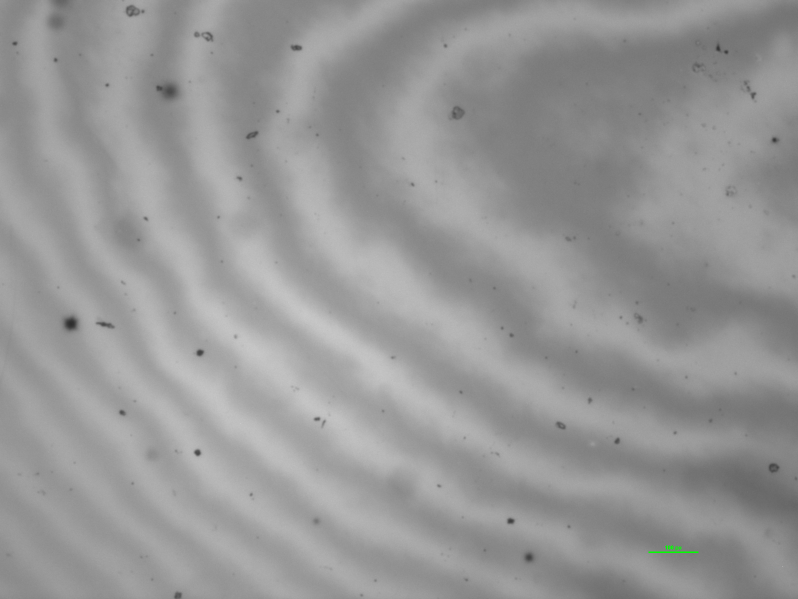
\includegraphics[scale=0.4]{obrazky/puvodni.png}
	\label{fig:puvodni}
	\caption{Původní snímek}
	\end{figure}
	
	\begin{figure}[!htb]
	\centering
	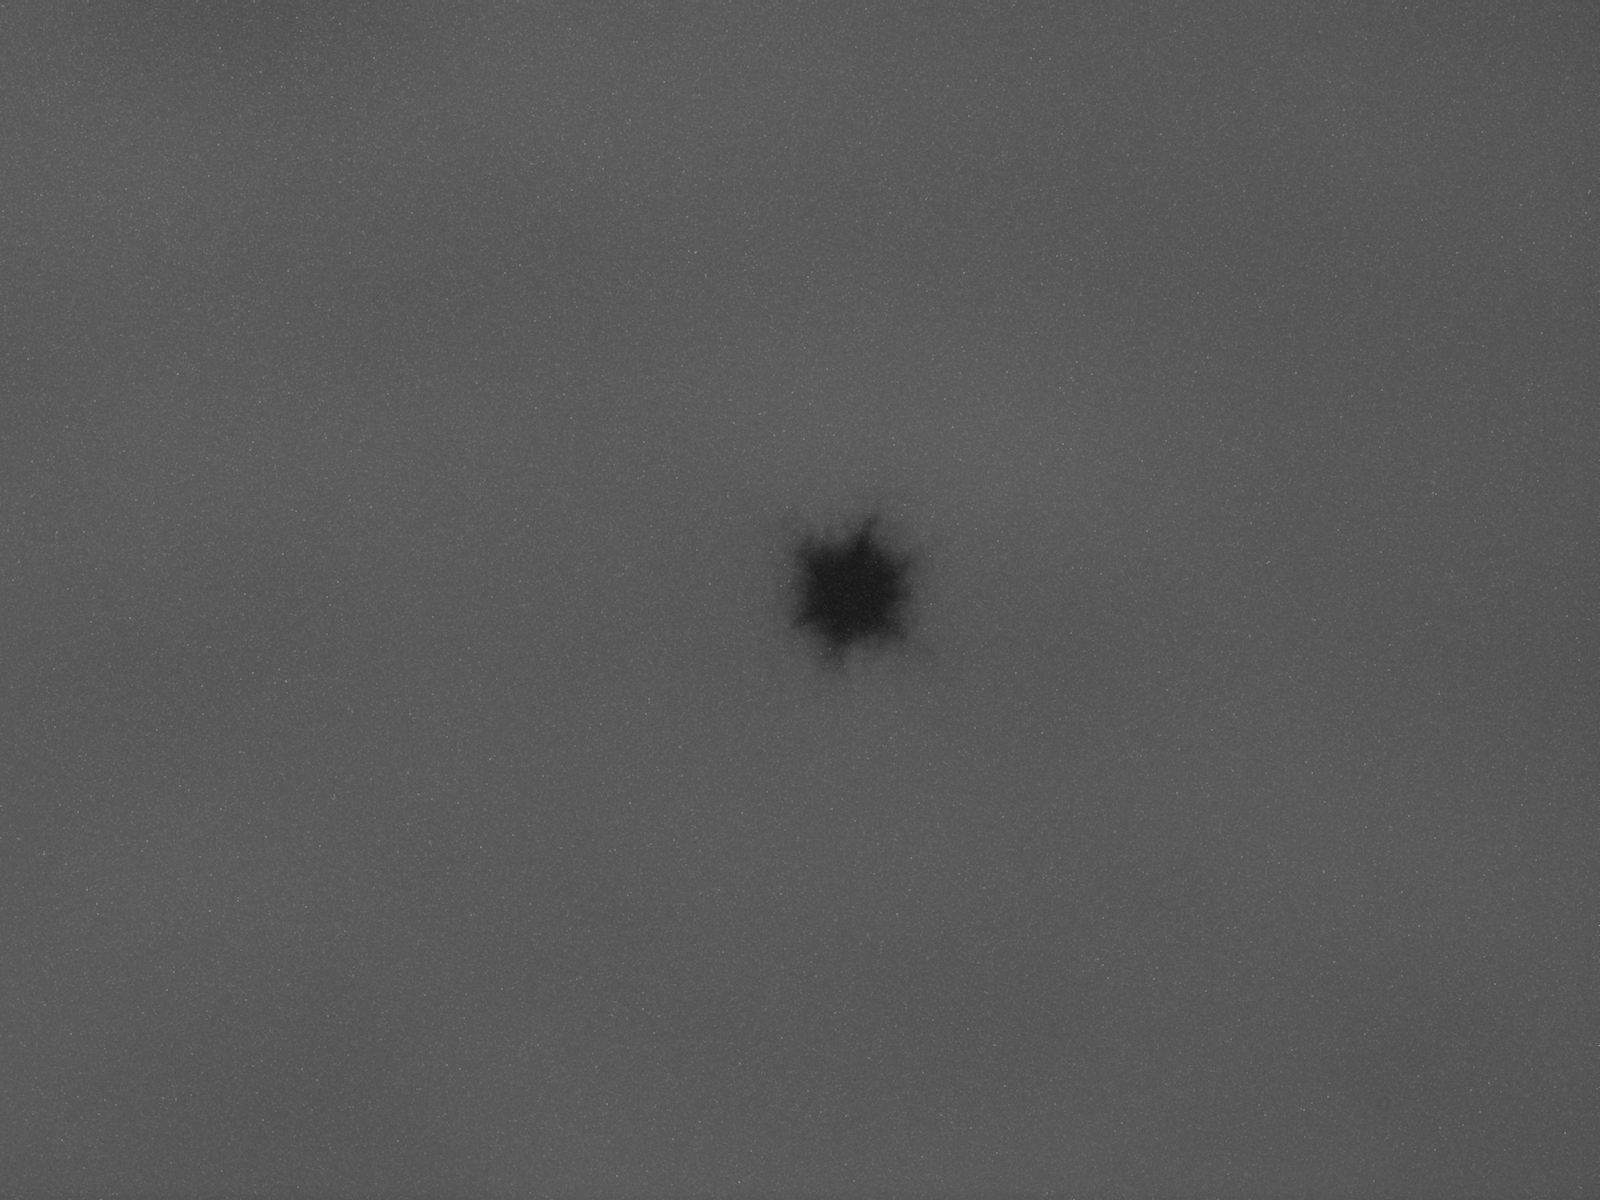
\includegraphics[scale=0.12]{obrazky/konvoluce.png}
	\label{fig:konvoluce}
	\caption{Konvoluce}
	\end{figure}	

	Dle histogramu původního snímku na obrázku 3.3 si lze povšimnout, že většina obrazových bodů na stupnici jasu od 0 do 255 nabývá hodnot v~intervalu přibližně od 100 do 200. Budeme uvažovat, že v~ostatních snímcích v~sekvenci je přibližně stejné rozložení hodnot jasu. Vzhledem k tomu, že konvoluce se jeví tmavé oproti ostatním obrazovým bodům snímku, zvýrazněním tmavých odstínů bychom docílili \uv{vystoupení} konvolucí. Naším cílem bude \uv{sjednotit} hodnoty vysokých jasů, tj. jasy vyšší než zvolená hodnota nabudou nejvyššího jasu (255), čímž potlačíme šum, jehož jas nabývá vysokých hodnot (např. vlny). Zbylé hodnoty \uv{roztáhneme} po celém intervalu 0 až 255, abychom... Hodnotu, kterou zvolíme jako mezní, určíme na intervalu od 100 do 150 (150 je \uv{vrchol} histogramu) tak, aby ve snímku zůstaly objekty \uv{podezřelé} z~konvolucí a zároveň bylo potlačeno co nejvíce šumu. Na obrázcích 3.4 až 3.6 vidíme výsledné snímky s~mezními hodnotami 100, 150 a 125. Při mezní hodnotě 100 je na snímku stále hodně viditelných vln, při hodnotě 150 je naopak možné, že některé konvoluce \uv{zmizely}. Mezní hodnota 125 se jeví jako dobrý kompromis.
	
	\begin{figure}[!htb]
	\centering
	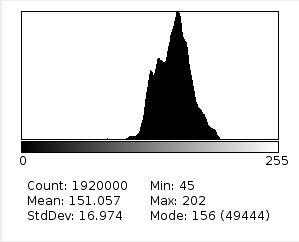
\includegraphics[scale=0.65]{obrazky/puvodni_histogram.png}
	\label{fig:puvodni_histogram}
	\caption{Histogram původního snímku}
	\end{figure}
	
	\begin{figure}[!htb]
	\centering
	
\includegraphics[scale=0.1]{obrazky/roztazeni_jasu_0_100.png}
	\label{fig:jas_0_100}
	\caption{Sjednocení vysokých jasů s~mezní hodnotou 100 a roztažení}
	\end{figure}	
	
	\begin{figure}[!htb]
	\centering
	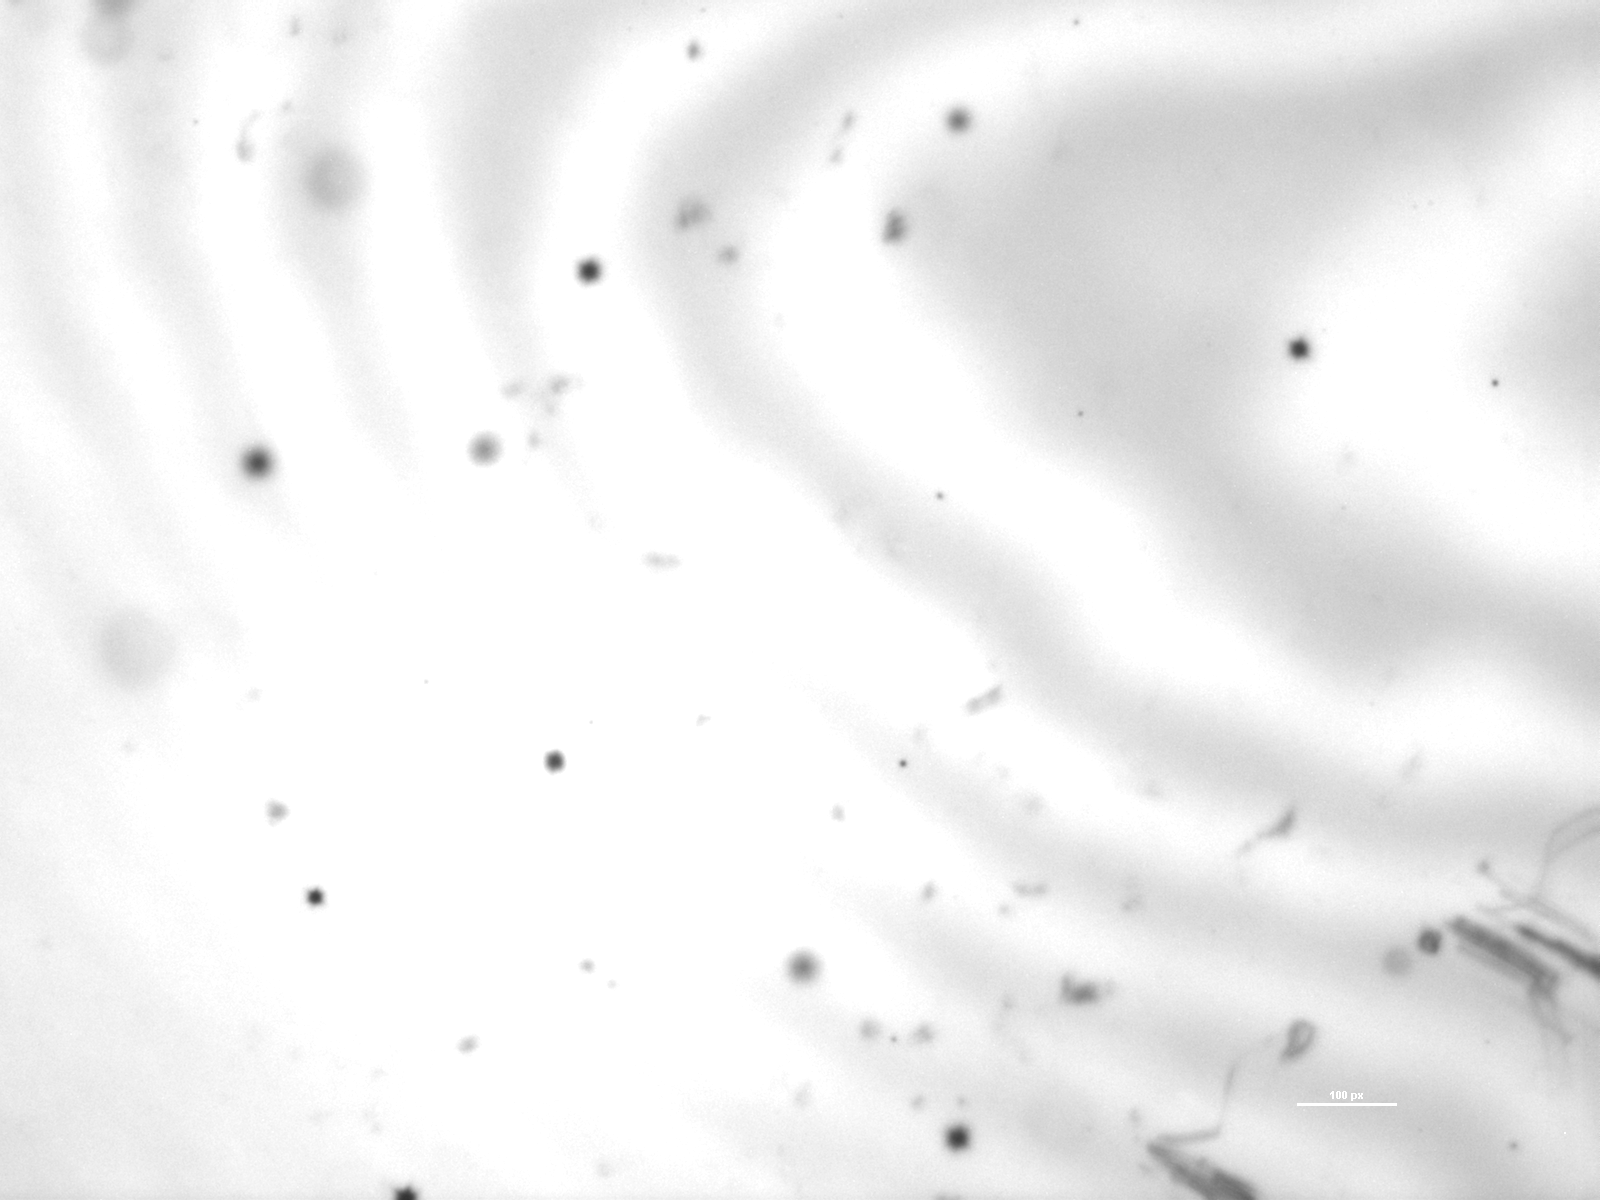
\includegraphics[scale=0.1]{obrazky/roztazeni_jasu_0_150.png}
	\label{fig:jas_0_150}
	\caption{Sjednocení vysokých jasů s~mezní hodnotou 150 a roztažení}
	\end{figure}
	
	\begin{figure}[!htb]
	\centering
	
\includegraphics[scale=0.1]{obrazky/roztazeni_jasu_0_125.png}
	\label{fig:jas_0_125}
	\caption{Sjednocení vysokých jasů s~mezní hodnotou 125 a roztažení}
	\end{figure}				
	
	Zvýraznění tmavých odstínů (včetně konvolucí) 
		a) Lineární transformace - posunutí histogramu: "sjednocení" vysokých jasů, eliminace "šumu"; roztažení histogramu: zvýšení kontrastu, došlo ke "zvýraznění" konvolucí, ale i nečistot na vzorku 
		b) Normování histogramu - složité hledání normovací funkce
		
	Prahování
	\section{Detekce konvolucí}


\chapter{Popis implementace}
Volba programových prostředků: OpenCV verze 2.4 (hlavní verze, snadno dostupná na všech platformách, doporučení???)
	Cleaner - vtvoří šedotón, 

\chapter{Uživatelská dokumentace}
	\section{SW požadavky}
	
	\section{Adresářová struktura odevzdávaného souboru}	
	
	\section{Spuštění a ovládání aplikace}	

\chapter{Závěr}
Cílem této semestrální práce bylo vytvořit aplikaci pro detekci konvolucí.

\end{document} 
